\section{Введение}
\label{sec:intro}

Распределенные системы, основанные на принципах параллельной обработки и разделения задач, значительно повышают эффективность и масштабируемость при работе с большими объемами данных. Одним из ведущих подходов в архитектуре таких систем является технология MapReduce \cite{mapreduce}, первоначально разработанная Google для индексации веб-страниц и обработки больших массивов информации, распределенных по множеству серверов.

Технология MapReduce организована вокруг двух основных функций: Map и Reduce. Функция Map принимает входные данные и преобразует их в промежуточные пары ключ-значение, которые затем агрегируются по ключам и передаются функции Reduce. Задача функции Reduce заключается в суммировании или иной форме обработки всех промежуточных значений, связанных с каждым ключом, для генерации конечного результата. Этот подход позволяет распределять обработку данных между множеством узлов, тем самым резко увеличивая производительность и обеспечивая горизонтальное масштабирование.

С другой стороны, существует задача описания бизнес-логики для обработки данных. Для решения подобных задач часто применяется методика разработки специализированных процессов - pipeline-ов. В рамках этой методики используется код, который определяет граф обработки данных. Эта структура определяет путь, по которому данные перетекают из одной системы в другую. В процессе такого перемещения данные могут подвергаться различным изменениям: обогащение путем интеграции дополнительной информации, или фильтрации, когда из потока удаляются нерелевантные или избыточные данные. Эти процессы помогают оптимизировать качество и структуру данных, делая их более подходящими для анализа и отчетности.

Существует два вида обработки больших объемов данных: batch и streaming.

Batch-обработка подразумевает работу с большими объемами данных, которые были предварительно сохранены в некотором хранилище. Это означает, что все данные уже подготовлены и доступны для обработки до начала выполнения pipeline-а. При таком подходе основной акцент делается на пропускную способность системы, так как инфраструктура должна быть рассчитана на выполнение сложных и трудоемких вычислений. Примером batch-обработки может служить анализ и построение выжимки из поисковых сессий пользователя за определенный день.

Важно отметить, что в процессе batch-обработки особое внимание уделяется не только скорости обработки больших данных, но и их последующей оптимизации для хранения и анализа. Например, после обработки данных о поисковых сессиях могут быть выделены ключевые метрики, которые затем используются для улучшения пользовательского опыта или оптимизации поисковых алгоритмов. Таким образом, качество обработки данных напрямую влияет на эффективность последующих бизнес-процессов.

Streaming-обработка данных означает, что данные поступают в систему порциями, известными как micro-batch, при этом полный объем данных неизвестен на момент запуска pipeline-а. В таких системах особенно важно уделять внимание времени, необходимому для обработки каждой такой порции. Это требует от инфраструктуры возможности быстро реагировать на потоковые данные и эффективно их обрабатывать, чтобы минимизировать задержки и обеспечить актуальность обрабатываемой информации. Примером использования streaming-обработки может служить агрегация данных о последних поисковых запросах пользователя, что позволяет предоставлять релевантные и своевременные результаты.

Помимо прочего два рассмотренных подхода объединяет то, что логика процессинга данных не зависит от способа обработки. Действительно, в случае batch процессингов данные могут быть обогащены более сложно вычислимыми статистиками. Однако с точки зрения, например, библиотеки для выражения логики на некотором языке программирования логика может быть представлена композицией функций многих входов и выходов. Более точная классификация такова: произвольные функции, модифицирующие, фильтрующие или мультиплицирующие данные (Map) и функции группировки (Reduce) по выделенному из данных ключу \cite{mapreduce}.

Благодаря использованию набора простых и понятных примитивов, появляется возможность разработки универсальной библиотеки, которая может предложить общий API для создания разнообразных процессов обработки данных. В результате такого подхода в компании Яндекс была разработана и реализована библиотека под названием Roren \cite{roren}.

\newpage
\subsection{Постановка задачи}

Инструмент должен решать задачу тестирования распределенной системы, внутри которой исполняется код студента.

Распределенную систему мы представим в виде набора узлов, объединенных в общую сеть. Узлы могут коммуницировать друг с другом только с помощью отправки сообщений.

Сеть мы считаем асинхронной и недетерминированной – она может произвольно задерживать и переупорядочивать отправляемые узлами сообщения. Если система будет корректно работать в асинхронной сети, то и в реальной, частично синхронной сети тоже.

Внутри узла исполняются недетерминированные программы. Также узлы могут отказывать, то есть перезагружаться в произвольные моменты и/или навсегда отключаться.

Мы считаем, что набор узлов системы реализует некоторый распределенный сервис, с которым клиенты взаимодействуют через протокол RPC. 

Клиенты тоже являются узлами сети. 

Они посылают системе запросы и получают ответы, в результате возникает конкурентная история, состоящая из отрезков запросов (рис.~\ref{fig:history_example}). Свойства системы формулируются как утверждения про допустимые истории, которые может порождать система.

\begin{figure}[h]
    \centering
    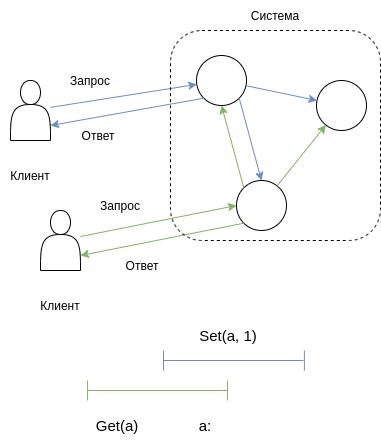
\includegraphics[width=0.5\textwidth]{img/task.png}
    \caption{Пример истории запросов}
    \label{fig:history_example}
\end{figure}

В данной работе нас прежде всего интересует задача репликации, так что распределенный сервис  представляет собой хранилище данных с операциями Set и Get, а свойство, которое мы ожидаем от системы – модель согласованности \cite{consistency}, в первую очередь – линеаризуемость \cite{linearizability}.

Наконец, сформулируем задачу – по реализации узлов системы проверить выполнение заявленных свойств независимо от поведения сети между узлами, часов и т.д.


\newpage
\subsection{Цель работы}

Цель работы состоит в реализации части библиотеки Roren, отвечающей за перевод и выполнение pipeline-ов поверх YT. Компонент должен позволять запускать произвольные графы обработки данных, выражаемые операциями Map/Reduce.

Получившаяся реализация в сравнении с текущей должна:
\begin{itemize}
    \item Переводить pipeline-ы в графы с меньшим количеством YT операций
    \item Иметь расширяемый на более сложные YT операции алгоритм трансляции
\end{itemize}


\newpage
\subsection{План работы}

Во второй главе мы рассмотрим дизайн библиотеки Roren: от API pipeline-ов до запуска YT операций.

В третьей главе рассмотрим реализацию компонента, производящего трансляцию. Мы изложим этапы перевода roren графа в граф YT операций, алгоритм трансляции, и детально остановимся на компоненте оптимизатора.

В четвертой главе посмотрим на примеры графов и их трансляций, обсудим тестирование.

В последней главе мы поговорим о результатах работы и обсудим пути развития компонента.

